\documentclass[../main.tex]{subfiles}

\begin{document}

\begin{tikzpicture}

\pie [rotate = 180, text=legend]
    {62/\TeX\ Live and Mac\TeX,
     32/MiK\TeX\ and Pro\TeX t, 6/Other \TeX}

\end{tikzpicture}

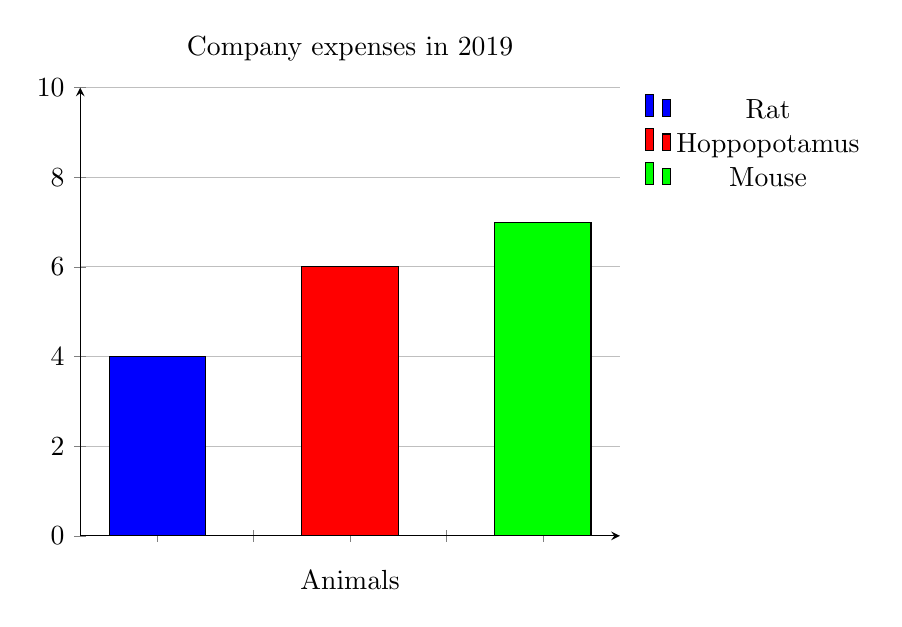
\begin{tikzpicture}
\begin{axis}[
    ybar,
    title={Company expenses in 2019},
    legend style={draw=none},
    legend pos = outer north east,
%   nodes near coords,
    axis y line=left,
    ymin=0,
    ymax=10,
    ymajorgrids,
    axis x line=bottom,
%   xticklabels={Rat,Hippopotamus,Mouse},
%   xtick={1,2,3}, % <-- added
    xticklabels={,,}, % remove xtick
    xlabel={Animals},
    every axis plot/.append style={ % <-- added
          bar width=.5,
          bar shift=0pt,
          fill},
    enlarge x limits=0.2, ]
        \addplot[fill=blue] coordinates {(1,4)};
        \addplot[fill=red] coordinates {(2,6)};
        \addplot[fill=green] coordinates {(3,7)};
\legend{Rat, Hoppopotamus, Mouse};
\end{axis}
\end{tikzpicture}


%\onlyinsubfile{\biblio}
\end{document}
